\section{Background}  \label{Background}



\subsection{Autonomous Driving Systems} \label{Background:AutonomousDrivingSystems}

% thesis: Autonomous Driving Systems have high safety requirements.

Autonomous Driving Systems (ADS), defined by the Society of Automotive Engineers (SAE) as the hardware and software that are collectively capable of performing the entire dynamic driving task (DDT) on a sustained basis, should have a high safety requirements.
This term is used to describe the three most advanced Levels 3 (Conditional), 4 (High), and 5 (Full) driving automation system.

Additionally, ADS must be capable of operating under diverse operational conditions, defined as the operational design domain (ODD). The ODD includes, but is not limited to, environmental, geographical, and time-of-day conditions.
While operating under these diverse conditions, ADS can experience DDT performance-relevant system failures that prevent it from reliably performing the DDT on a sustained basis.
In such cases, the ADS must issue a request to intervene, either for the user to perform the DDT or for the system to achieve a minimal risk condition.

At Level 3, a DDT fallback-ready user is expected to take over the DDT when a DDT performance-relevant system failure occurs or when the ADS is about to leave its operational design domain (ODD). This user must be receptive and able to resume DDT performance when alerted to do so.
For example, a Level 3 ADS experiences a DDT performance-relevant system failure in one of its radar sensors, which prevents it from reliably detecting objects in the vehicle's pathway. The ADS responds by issuing a request to intervene to the DDT fallback-ready user. The ADS continues to perform the DDT, while reducing vehicle speed, for several seconds to allow time for the DDT fallback-ready user to resume operation of the vehicle in an orderly manner. It is important to highlight that a key expectation for Level 3 ADS is the capability of continuing to perform the DDT for at least several seconds after issuing the fallback-ready user with a request to intervene.

For Levels 4 and 5 ADS, if a driving automation system can perform the entire DDT and DDT fallback either within a prescribed ODD (Level 4) or in all driver-manageable on-road operating situations (Level 5), then any users present in the vehicle while the ADS is engaged are passengers. For example, if a Level 4 ADS experiences a DDT performance-relevant system failure in one of its computing modules, it transitions to DDT fallback by engaging a redundant computing module(s) to achieve a minimal risk condition.

The high safety requirements defined by SAE imply significant robustness expectations for ADS. This means that an ADS should be capable of, first, performing the DDT for a few seconds following a performance-relevant system failure until DDT fallback, and second, in the case of Levels 4 and 5, it must be able to reach a minimal risk condition despite such a system failure\cite{sae:j3016:2021apr}.

Automated Driving Systems (ADS) should be capable of perceiving data from different sources. The Dynamic Driving Task (DDT) is defined as all real-time operational and tactical functions required to operate a vehicle in on-road traffic. Object and Event Detection and Response (OEDR) refers to the subtasks of the DDT that include monitoring the driving environment (detecting, recognizing, and classifying objects and events, and preparing to respond as needed) and executing an appropriate response to such objects and events (i.e., actions required to complete the DDT and/or DDT fallback). Performing the OEDR is necessary to complete the DDT and DDT fallback, and the capability of a Driving Automation System to handle OEDR allows it to be classified as Level 3 automation or higher.


The DDT encompasses all real-time operational and tactical functions required for driving, including lateral and longitudinal motion control, and Object and Event Detection and Response (OEDR).




ADS term is used to describe the last three and the most advanced SAE Levels 3 (Conditional), 4 (High), and 5 (Full) driving automation. ADS operate under high safety requirements, therefore crash mitigation and avoidance capability is part of ADS functionality.

An Automated Driving System (ADS) refers to the hardware and software
collectively capable of performing the entire Dynamic Driving Task (DDT)
on a sustained basis, applicable to SAE Levels 3 (Conditional), 4
(High), and 5 (Full) driving automation{ \textsuperscript{} }.

Unlike
lower levels of automation which merely assist a human driver, an ADS
takes full responsibility for operating the vehicle within its specified
Operational Design Domain (ODD), if applicable{ \textsuperscript{} }.

This transfer of complete, real-time operational and tactical control {
\textsuperscript{} } inherently necessitates that Autonomous Driving
Systems operate under high safety requirements. The complexity involved
in perceiving the environment, making safety-critical decisions, and
executing maneuvers without human oversight demands rigorous design,
validation, and operational safeguards, particularly concerning the
system\textquotesingle s ability to manage unforeseen events and
internal malfunctions safely{ \textsuperscript{} }. { ~ }

A critical aspect supporting the high safety requirements for ADS
revolves around \textbf{Failure Mitigation and Safe States}. ADS are
complex integrations of hardware, software, and sensors, components of
which are inevitably subject to DDT performance-relevant system failures
-- malfunctions preventing the reliable performance of the driving task
{ \textsuperscript{} } (P1). To uphold safety during such occurrences,
ADS must incorporate predefined strategies for DDT fallback{
\textsuperscript{} }. This involves the system responding appropriately
to a failure or ODD exit, which for Level 4 and 5 systems means the ADS
must automatically achieve a Minimal Risk Condition (MRC) -- a stable,
stopped state designed to reduce crash risk{ \textsuperscript{} }. For
Level 3 systems, fallback may involve issuing a timely request to
intervene to a fallback-ready user, expecting them to resume the DDT or
achieve an MRC { \textsuperscript{} } (P2). During such a transition in
Level 3, the ADS is expected to continue performing the DDT safely for a
period to allow the user time to respond appropriately {
\textsuperscript{} } (P3). Consequently, robust failure detection
capabilities coupled with comprehensive mitigation strategies are
essential for ADS to reliably transition the vehicle to an appropriate
safe state -- whether that is under user control following a fallback
request or an automatically achieved MRC -- upon system malfunction or
performance degradation { \textsuperscript{} } (C1). { }


There's an expectation of 

State-of-the-art ADS employ a wide variety of sensors, often with redundancy, to ensure safety. These sensors can be categorized based on their purpose. In this thesis, we focus on exteroceptive sensors, which are primarily used for perceiving the surrounding environment to accomplish tasks necessary for the ADS.





% goal: explain relevance between ADS and video object detection task

Autonomous vehicle are complex on multi-sensor perception, integrating data from various sources such as LiDAR, cameras, and radar to create a comprehensive understanding of the environment.

Definition of autonomous driving systems. Explain architecture.

Type of sensors in ADS.

\subsection{Sensors} \label{Background:Sensors}

% goal: explain relevance between sensors and video object detection task


\subsection{Video Object Detection} \label{Background:VideoObjectDetection}

% Object detection definition. Deep learning pushed performance of single image object detection.

Object detection is a foundational challenge in computer vision and has been a subject of research for several decades \cite{fischlerRepresentationMatchingPictorial1973}. The goal of the object detection task is to find object(s) of given description in images and videos. Advancements in deep learning techniques to learn feature representations \cite{hintonReducingDimensionalityData2006, lecunDeepLearning2015} have made it possible to achive remarkable progress in single-image object detectors \cite{girshickRichFeatureHierarchies2014a}.

% State-of-the-Art
% Still-image detector

Due to similarity beetwen object detection on image and video, the simplest approach to tackle a video object detection is to use a single-image object detector, so treat each video frame as an independent image. However, this approach is naive because it completely ignores temporal and contextual information of the video. A still image detector is not able to consistently predict objects acrsso all video frames due to numerouse artefactos and biases in the video (e.g., motion blur, occlusion, unusual position).

% Postprocessing (not e2e)

%One intuition to improve temporal consistency is to propagate detection results to neighbor frames to reduce sudden changes of detection results.

%In this work we propose a simple extension of single image object detection to help overcome these difficulties.

Another simple approach which improves temporal consistency of video object detections involves a postprocessing step after still image detector \cite{hanSeqNMSVideoObject2016, kangTCNNTubeletsConvolutional2018, kangObjectDetectionVideo2016}. Detections from adjecent frames are used to improve results of the current frame. At postprocessing step researches apply technich like non-maximum suppression (NMS) \cite{hanSeqNMSVideoObject2016} or optical flow \cite{kangTCNNTubeletsConvolutional2018, kangObjectDetectionVideo2016}. Although these methods show improvement over a stil image detector aproach, exploiting temporal information as postprocessing is sub-optimal since temporal and motion information are ignored during detector training.

% TODO: paper Multi-Class Multi-Object Tracking using  Changing Point Detection

% VIDEO DETECTION WITH ADDITIONAL MODELS

Another approach suggests to introduce motion and temporal information during training to form an end-to-end solution. In \cite{Lu_2017_ICCV} proposed to use a LSTM \cite{6795963} to refine the detection results together with association features which representation of the detected objects. This model is end-to-end and can be trained jointly with the object detector. This algorithm rely on objects association between adjacent frames therefore it is limited to short-term motion information and cannot handle long occlusions or unusual appearance of for a long time which is the same problem with algorithms based on postprocessing. Another work proposes a recurrent computation unit called spatial-temporal memory module (STMM) \cite{xiaoVideoObjectDetection2018} which uses a ConvGRU \cite{ballasDelvingDeeperConvolutional2016} to preserve a spacio temporal structure and show suggests the effectiveness of our memory: the longer the sequence, the more longer-range useful information is stored in the memory, which leads to better detection performance.

% Transformers

Transformers [32], [33], [34], [35], [36] have shown promising potential in computer vision. Especially, DETR [33], [34] simplifies the detection pipeline by modeling the object queries and achieving comparative performance with highly optimized CNN-based detectors.


Most architectures used by AI systems today are specialized. For instance, a 2D residual network might excel at processing images, but it's hardly ideal for other data types, such as the LiDAR point clouds or radar output used in ADS. Handling multiple data modalities, like the sounds and images that make up videos, presents even greater complexity and usually involves complex, hand-tuned systems built from many different parts, even for simple tasks. Real-world problems, such as building an ADS, possess these complexities, so there is a desperate need to build a simple yet effective, more general, and versatile architecture that can handle all types of data.


\subsection{General Purpose Perceiver Model} \label{Background:Perceiver}

Most architectures used by AI systems today are specialized. For instance, models presented in \ref{Background:VideoObjectDetection} built for the video object detection task might excel at processing 2D video frames, but they are hardly ideal for other data types, such as the LiDAR point clouds or radar output used in ADS. Handling multiple data modalities, like the sounds and images that make up videos, presents even greater complexity and usually involves complex, hand-tuned systems built from many different parts, even for simple tasks. Real-world problems, such as building an ADS, possess these complexities, so there is a desperate need to build a simple yet effective, more general, and versatile architecture that can handle all types of data.

Paper \cite{jaeglePerceiverGeneralPerception2021} introduces the Perceiver, a general-purpose architecture that is capable of processing different data types such as images, point clouds, audio, video, and, what is important, combinations of those to fuse together. The Perceiver builds upon the Transformer \cite{}, an architecture that uses an operation called "Attention" to map inputs into outputs \cite{}. While attention is simple and widely applicable, the way Transformers utilize attention can become memory expensive as the number of inputs grows. Consequently, Transformers perform well with inputs containing at most a few thousand elements, but common data forms like images and videos can easily comprise millions of elements. This fact poses a challenge to the generalist architecture: scaling the Transformer's attention operation to very large inputs without introducing domain-specific assumptions. The Perceiver addresses this by using attention to first encode the inputs into a small latent array. This latent array can then be processed further at a cost independent of the input's size, allowing the Perceiver's memory and computational needs to scale gracefully as the input size grows, even for particularly deep models. This "graceful growth" enables the Perceiver to achieve an unprecedented level of generality - it is competitive with domain-specific models on benchmarks based on images, 3D point clouds, and combined audio and images.

\begin{figure}
    \centering
    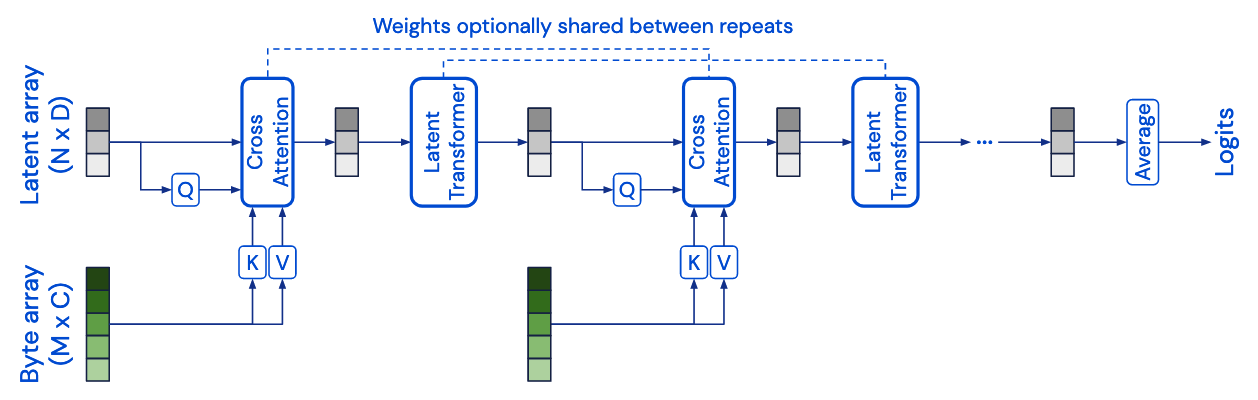
\includegraphics[width=\textwidth]{figures/figure_background_perceiver_architecture.png}
    \caption{The Perceiver is an architecture based on attentional principles that scales to high-dimensional inputs such as images, videos, audio, point-clouds, and multimodal combinations without making domain-specific assumptions. The Perceiver uses a cross-attention module to project an high-dimensional input byte array to a fixed-dimensional latent bottleneck (the number of input indices M is much larger than the number of latent indices N ) before processing it using a deep stack of Transformer-style self-attention blocks in the latent space. The Perceiver iteratively attends to the input byte array by alternating cross-attention and latent self-attention blocks \cite{jaeglePerceiverGeneralPerception2021}.}
    \label{fig:figure_background_perceiver_architecture}
\end{figure}

The Perceiver architecture is built from two components: (i) a cross-attention module that maps a byte array (e.g. an pixel array) and a latent array to a latent array, and (ii) a Transformer tower that maps a latent array to a latent array \cite{jaeglePerceiverGeneralPerception2021}. The Perceiver architecture is illustrated in Figure \ref{fig:figure_background_perceiver_architecture}. The model can be interpreted as a recurrent neural network (RNN), but unrolled in depth using the same input, rather than in time. The main challenge addressed by the architecture's design is scaling attention architectures to very large and generic inputs. The Perceiver circumvents this quadratic bottleneck through its cross-attention module. Attention is applied directly to the inputs by introducing an asymmetry into the attention operation. First, note that for $Q \in \mathbb{R}^{M \times D}$, $K \in \mathbb{R}^{M \times C}$, and $V \in \mathbb{R}^{M \times C}$, (where $C$ and $D$ are channel dimensions) the complexity of the $QKV$ attention operation - essentially, $softmax(QK^T)V$ - is $O(M^2)$, as it involves two matrix multiplications with matrices of large dimension $M$. Authors introduced asymmetry: while $K$ and $V$ are projections of the input byte array, $Q$ is a projection of a learned latent array with index dimension $N \ll M$, where the latent's index dimension $N$ is a hyperparameter. The resulting cross-attention operation has complexity $O(MN)$. This design allows Perceiver-based architectures to make use of much deeper Transformers than efficient Transformers that use linearcomplexity layers, without relying on domain-specific assumptions. This is because a Transformer built on bytes has complexity O(LM 2) while a latent Transformer has complexity O(LN 2) (where $N \ll M$), when considered as a function of the number of layers $L$ in addition to index dimensionality. The overall architecture's complexity thus becomes $O(MN + LN^2)$ for a latent Transformer with $L$ layers, and this is key: by decoupling the input size and the depth, we can add additional Transformer layers at a cost that’s independent of the input size.

However, because the original Perceiver produced only one output per input, it was not as versatile as researchers required. The Perceiver architecture is quite we want to modify it to be more like a recurrent module.